
%------------------------------------
\subsection{連続型特徴量(Continuous features, CF)}
%------------------------------------
従来手法\citep{caplan2015risk}では,距離とカーネル密度推定値による連続型特徴量を離散化するが,
CFでは離散化せず連続型特徴量のままRTMの予測変数とする.

%------------------------------------
\subsection{負の冪での変換(Negative Exponent, NE)}
%------------------------------------
NEでは,CFの特徴量の連続化の発展として,距離特徴量$d$を負の冪(\ref{inverse})式で変換する.

\begin{equation}\label{inverse}
  \abs{d}^{-\gamma}
\end{equation}
ここで,$\gamma$は指数を決定する正のパラメータである.

%------------------------------------
\subsection{ラプラス分布関数での変換(Laplace distribution, LD)}
%------------------------------------
LDでは,CFでの特徴量の連続化の発展として,距離特徴量$d$を
規格化定数を除いたラプラス分布関数(\ref{laplace})式で変換する.

\begin{equation}\label{laplace}
  \exp \left( -\frac{\abs{d}}{\sigma}\right)
\end{equation}
ここで,$\sigma$はラプラス分布の尺度を決定するパラメータである.


%------------------------------------
\subsection{ガウス関数での変換(Gauss function,GF)}
%------------------------------------
GFでは,CFでの特徴量の連続化の発展として,距離特徴量$d$をガウス関数

\begin{equation}\label{gauss}
  \exp \left(-\frac{d^2}{2\sigma^2} \right) \notag
\end{equation}
で変換する.ここで,$\sigma$はガウス関数の尺度を決定するパラメータである.

% ------------------------------------
\subsection{2次元ガウス特徴量(Two-dimensional Gaussian feature, TG)}
%------------------------------------
TGでは,図\ref{fig:TG-knn}のようにあるグリッドセル中心点から地理的リスク要因の
近傍点を求め,ガウス分布を生成する.
このガウス分布により,あるグリッドセル中心点における,局所的な地理的リスク要因の分布傾向を考慮した
新たな特徴量を提案する.
図\ref{fig:TG-knn}の左右の図は同じ平均を持つガウス分布である.
左図は近傍点が偏りなく分布していて,グリッドセル中心点の確率密度関数の値は大きくなる.
右図は近傍点が偏って分布しているため,グリッドセル中心点での確率密度関数の値は小さくなる.

特徴量構成方法の詳細は,$l$番目のグリッドセル中心点$x_l$に対して,
kNN\citep{bishop2007}により取得したある地理的リスク要因の近傍点$K$個から2次元ガウス分布を求め,
その確率密度関数を表現する.
$l$番目のグリッドセルに対して 
kNNを用いて求めた\( K \) 個の近傍点を\( \{ x_{l1}, x_{l2}, \dots, x_{lK} \} \) とする.
各点 \( x_i \) は2次元座標 \( x_i = (x_{i1}, x_{i2})^\top \) を持つとする.
これらの近傍点の平均 \( \mu_l \),共分散行列\( \Sigma\) は
(\ref{TG-mu})式,(\ref{TG-Sigma})式で計算される.

\begin{equation}\label{TG-mu}
  \mu_l = \frac{1}{K} \sum_{i=1}^{K} x_{li}
\end{equation}

\begin{equation}\label{TG-Sigma}
  \Sigma_l = \frac{1}{K} \sum_{i=1}^{K} (x_{li} - \mu_l)(x_{li} - \mu_l)^\top
\end{equation}
グリッドセル中心点 \( x_l \) における確率密度関数の値は(\ref{TG-pdf})式のように表される.

\begin{equation}\label{TG-pdf}
p(x_l) = \frac{1}{2\pi |\Sigma_l|^{1/2}} \exp \left( -\frac{1}{2} (x_l - \mu_l)^\top \Sigma_l^{-1} (x_l - \mu_l) \right)
\end{equation}
この値を2次元ガウス特徴量として利用することで,各グリッドセル中心点 \( l \)での
局所的な地理的リスク要因の分布情報をモデルに組み込む.

\begin{figure}[H]
  \centering % 図を中央寄せにする
  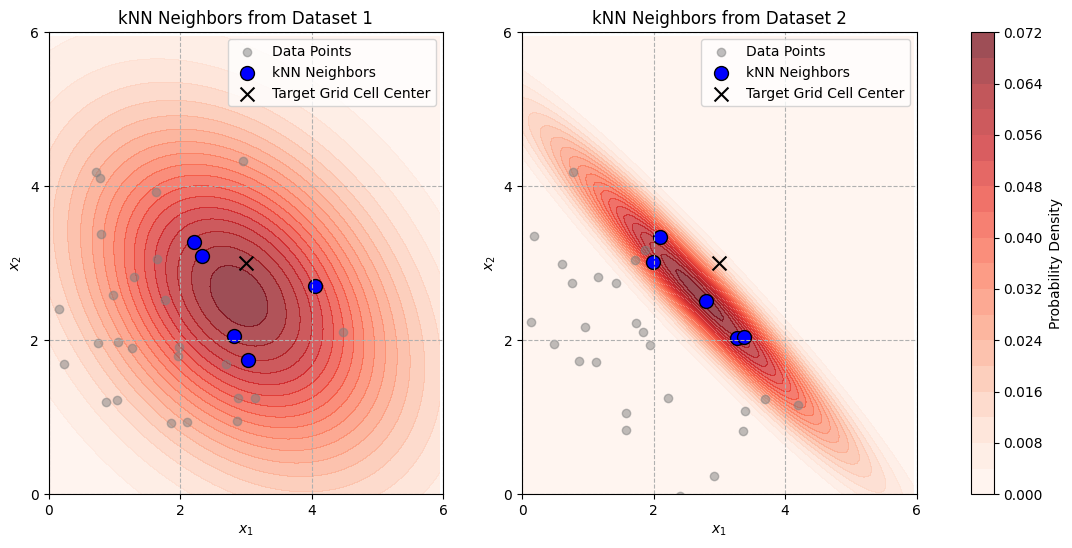
\includegraphics[scale=0.3]{./util-fig/TG-knn.png}
  \caption{kNNによるガウス分布}
  \label{fig:TG-knn}
\end{figure}
% ------------------------------------
\subsection{ガウス関数での変換と2次元ガウス特徴量(GF+TG)}
%------------------------------------
距離特徴量をガウス関数によって変換するGFと,
2次元ガウス特徴量を生成するTGを並列に入れた特徴量構成法をGF+TGとする.